\chapter{Programsko ostvarenje}

Praktičan dio rada izveden je kroz desktop aplikaciju s grafičkim sučeljem. Aplikacija može pokrenuti ranije opisane algoritme i usporediti rezultate grupiranja prema evaluacijskim mjerama na odabranim skupovima podataka. Aplikacija je napisana u programskom jeziku Python \cite{van1995python}. Python je pogodan za rješavanje problema vezanih uz obradu i analizu podataka. Kroz njega je dostupno mnogo biblioteka koje su napisane za analizu specifičnih problema. Konkretne implementacije napravljene su u programskim jezicima kao što je C++ što značajno ubrzava izvođenje u odnosu kada bi implementacija bila napravljena u Pythonu. Nakon što se željeni algoritam izvrši, kroz Python se pružaju bogate mogućnosti u povezivanju s drugim bibliotekama koje se koriste i obradi dobivenih rezultata i vizualizaciji.

Za izradu grafičkog sučelja korišten je Pythonov paket tkinter. Za analizu rezultata i grafički prikaz korištena je biblioteka Matplotlib, dok su za rad s mrežama i njihovom analizom korištene tri biblioteke: SNAP, NetworkX i cdlib. Alati za analizu mreža moraju ispunjavati određene pretpostavke u radu. Moraju pružiti bogate funkcionalnosti za rad i obradu velikih mreža koje mogu imati milijune čvorova te implementirati algoritme koji će ih analizirati. Moraju biti u kompaktnom obliku kako bi memorijsko zauzeće bilo što manje	budući da su mnogi algoritmi ograničeni upravo memorijskim kapacitetima.

\section{Biblioteka SNAP}
Stanford Network Analysis Platform biblioteka (SNAP) \cite{leskovec2016snap} je sustav za analizu grafova i mrežnih sustava. Napisana je u programskom jeziku C++ te je optimizirana kako bi imala najbolje moguće performanse i na prikladan način predstavljala grafove. Biblioteka je osmišljena tako da su algoritmi koji se izvršavaju neovisni od tipa grafa ili mreže i njihove konkretne reprezentacije. Tako većina metoda radi za gotovo bilo koji tip grafa te je tim svojstvom dobivena mogućnost da se velike mreže, sa stotinama milijuna čvorova i milijardama bridova, dobro skaliraju. Kroz modul Snap.py većina SNAP funkcionalnosti dostupna je u programskom jeziku Python čime se olakšava njezino korištenje kroz napredne mogućnosti tog jezika. Za osnovne funkcionalnosti SNAP ne zahtjeva dodatne biblioteke. 

\begin{figure}
	\makebox[\textwidth][c]{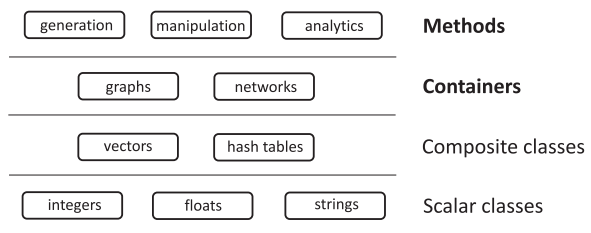
\includegraphics[width=0.8\textwidth]{images/snap-slojevi.png}}
	\caption{Slojevi u dizajnu implementacije SNAP biblioteke \cite{leskovec2016snap}}
	\label{fig:SNAP_design}
\end{figure}

Implementacijski dizajn biblioteke podijeljen je u četiri sloja, što je prikazano na slici \ref{fig:SNAP_design}. U donjem sloju nalaze se klase skalara kao što su cijeli ili decimalni brojevi i stringovi. U njih se pohranjuju osnovni podaci o svakom vrhu. Iznad njega nalazi se sloj sa kompozitnim kolekcijama podataka kao što su vektori i hash tablice. One moraju efikasno pristupati pohranjenim elementima i iterirati kroz njih kako bi se obavljale operacije potrebne za rad algoritama. U sljedećem čvoru su klase koje su implementacije grafova te sadrže metode za održavanje strukture, odnosno dodavanje ili brisanje čvorova. Navedene metode moraju biti brze i učinkovite. Na vrhu se nalazi sloj sa metodama koji implementira algoritme i oslanja se na niže slojeve koji obavljaju operacije u pojedinim koracima.

Biblioteka se osim za izvor stvarnih primjera skupova podataka koristi i za pokretanje Girvan-Newman algoritma te kao rezultat vraća vrijednost modularnosti i pronađene zajednice. Poziva se sljedećom naredbom:
\begin{verbatim}
	modularity, communities = G.CommunityGirvanNewman().
\end{verbatim} 



\section{Biblioteka NetworkX}
NetworkX \cite{SciPyProceedings_11} je programska biblioteka jezika Python koja pruža alate za stvaranje, obradu i proučavanje strukture i ponašanja velikih mreža iz raznih područja primjene. Sadrži sučelje prema Pythonu i implementaciju brojnih tipova mreža i grafova kao što su jednostavni grafovi, usmjereni grafovi ili grafovi s paralelnim bridovima i petljama. Čvorovi mogu biti predstavljeni Python objektima koji implementiraju hash funkciju te mogu sadržavati proizvoljne podatke koji opisuju čvor.


Kompleksni algoritmi i numeričke operacije napisani su u jezicima C, C++ i FORTRAN. Biblioteka pruža mogućnosti rada sa raznim tipovima grafova, njihovom manipulacijom, konstrukcijom slučajnih modela te grafičkim prikazom grafova. Implementirani su algoritmi za računanje tipičnih svojstava grafa, npr. pronalaženje najkraćeg puta ili pronalaženja distribucije stupnjeva vrhova. Moguće je generirati mrežu sa small-world svojstvima prema Watts-Strogatz modelu na sljedećom naredbom, gdje su $N$ broj čvorova, $k$ broj susjeda i $p$ vjerojatnost prespajanja brida:
\begin{verbatim}
	G = nx.generators.watts_strogatz_graph(N, k, p).
\end{verbatim}
Biblioteka pruža potporu za rad sa raznim formatima ulaznih podataka te ako postoji ulazna datoteka koja sadrži graf zapisan pomoću liste susjedstva jednostavno se učitava na sljedeći način: 
\begin{verbatim}
	G = nx.read_adjlist(filename)
\end{verbatim}
Spremanje generiranog grafa u datoteku kao listu susjedstva izvršava se sljedećom naredbom:
\begin{verbatim}
	nx.write_adjlist(G, filename).
\end{verbatim}

Osim za pohranu grafova biblioteka NetworkX koristit će se za grafički prikaz manjih grafova pogodnih za vizualizaciju rješenja koje je algoritam pronašao. Graf sadrži redni broj čvora te su čvorovi različitih zajednica u različitim bojama. Primjer se može vidjeti na slici \ref{fig:drawing}. Iscrtavanje se poziva naredbom
\begin{verbatim}
	nx.draw(graph, pos = nx.spring_layout(graph), node_color=colorMap,
			with_labels=withLabels)
\end{verbatim}
kojoj se predaje graf, algoritam za razmještanje čvorova na zaslonu, mapa sa definiranim bojama za svaki čvor te logička varijabla kojom se uključuje ili isključuje oznake čvorova. 

\begin{figure}
	\makebox[\textwidth][c]{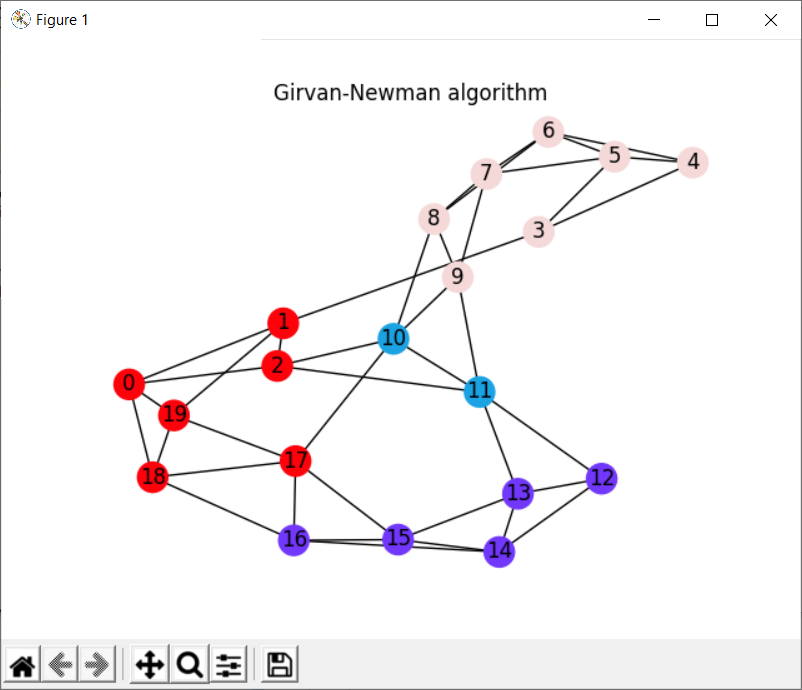
\includegraphics[width=0.8\textwidth]{images/draw-graph.png}}
	\caption{Grafički prikaz pronađenih zajednica u grafu Girvan-Newman algoritmom.}
	\label{fig:drawing}
\end{figure}

\pagebreak

\section{Biblioteka cdlib}
Community Discovery Library (cdlib) \cite{rossetti2019cdlib} je Python biblioteka za analizu i otkrivanje društvenih zajednica, stvorena na temelju grafovskih struktura podataka koje pružaju biblioteke NetworkX i Igraph. Biblioteka pruža implementacije raznih varijacija algoritama u području otkrivanje društvenih zajednica uključujući algoritme za pronalaženje nepreklapajućih zajednica, preklapajućih zajednica i neizrazitih zajednica gdje se za čvor računa razina kojom pripada zajednicama. Ukupno je implementirano 39 algoritama. Graf se definira preko strukture podataka koju nudi bilo koja od navedenih biblioteka te se nad njim pokreće algoritam iz cdlib biblioteke.

Biblioteka sadrži niz alata za usporedbu i evaluaciju kvaliteta pojednih grupa i čitavih rješenja koje algoritam pronalazi. Kada se izračunaju rješenja grupiranja za željenu mrežu tada cdlib omogućava evaluaciju koristeći mjere kvalitete, usporedbu sa alternativnim podjelama zajednica vizualizaciju rješenja za prikladne veličine grafova.

Iz cdlib biblioteke koristit će se implementacije za četiri algoritma detekcije zajednica: Louvain, Surprise, Leiden i Walktrap. Algoritmi se pokreću sljedećim naredbama:

\begin{verbatim}
	communities = algorithms.louvain(g_original)
\end{verbatim}


\begin{verbatim}
	communities = algorithms.surprise_communities(g_original)
\end{verbatim}

\begin{verbatim}
	communities = algorithms.leiden(g_original)
\end{verbatim}

\begin{verbatim}
	communities = algorithms.walktrap(g_original).
\end{verbatim}


Algoritmi kao rezultat vraćaju objekt razreda $NodeClustering$ koji sadržava informacije o pronađenim zajednicama, referencu na originalan graf, metapodatke o algoritmu koji se koristio, npr. ime algoritma i konfiguracijski parametri, zastavicu koja označava je li algoritam bio preklapajući ili nije te postotak čvorova koji su uključeni u grupiranje. Dobiveni objekt može se slati evaluacijskim funkcijama koje tada računaju rezultate mjera koje je algoritam pronađenom konfiguracijom zajednica ostvario.